% Clase de documento
\documentclass[letterpaper,12pt,oneside]{book}
% Paquetes
\usepackage[utf8]{inputenc}                                           % Codificación de caracteres
\usepackage[T1]{fontenc}                                              % Codificación de salida
\usepackage[spanish,es-nodecimaldot,es-tabla]{babel}                  % Idioma español
\usepackage{graphicx}                                                 % Para insertar imágenes
\usepackage[top=1in, left=0.9in, right=1.25in, bottom=1in]{geometry}  % Márgenes
\usepackage{tikz}                                                     % Para crear gráficos
\usepackage{tocloft}                                                  % Para personalizar la tabla de contenido
\usepackage{setspace}                                                 % Para el interlineado
\usepackage[backend=biber,style=numeric, sorting=none, doi=false, url=false]{biblatex}                    % Para la bibliografía
\usepackage{csquotes}                                                 % Para citas bibliográficas
\usepackage{amsmath}                                                  % Para ecuaciones matemáticas
\usepackage{amsfonts}
\usepackage{amssymb}
\usepackage[version=4]{mhchem}                                        % Para fórmulas químicas, especificando la versión
\usepackage{booktabs}                                                 % Para mejores líneas en tablas
\usepackage{longtable}                                                % Para tablas largas
\usepackage{siunitx}                                                  % Para el comando \SI y manejo de unidades
\usepackage{pdflscape} % Paquete para orientación horizontal
\usepackage{graphicx}  % Necesario para \centering en algunos casos
\usepackage{rotating} % Paquete para el entorno sidewaystable
\usepackage{subcaption}
\usepackage{float}
\usepackage{helvet}
\renewcommand{\familydefault}{\sfdefault}

\DeclareSIUnit\angstrom{\text {Å}}
\graphicspath{{./Imágenes/}}     % Ruta de las imágenes

% Archivo de bibliografía
\addbibresource{referencias.bib}

\begin{document}
%\onehalfspacing % O \doublespacing, para doble espaciado
%\doublespacing
    
\begin{titlepage}
    \thispagestyle{empty}
    \begin{minipage}[c][0.17\textheight][c]{0.23\textwidth}
        \begin{center}
            
\includegraphics[width=3.5cm, height=3.5cm]{Escudo-UNAM.pdf}
        \end{center}
    \end{minipage}
    \begin{minipage}[c][0.195\textheight][t]{0.725\textwidth}
        \begin{center}
            \vspace{0.3cm}
            \textsc{\large Universidad Nacional Aut\'onoma de M\'exico}\\[0.5cm]
            \vspace{0.3cm}
            \hrule height2.5pt
            \vspace{.2cm}
            \hrule height1pt
            \vspace{.8cm}
            \textsc{Facultad de Química}\\[0.5cm] %
        \end{center}
    \end{minipage}

    \begin{minipage}[c][0.81\textheight][t]{0.20\textwidth}
        \vspace*{5mm}
        \begin{center}
            \hskip2.0mm
            \vrule width1pt height13cm 
            \vspace{5mm}
            \hskip2pt
            \vrule width2.5pt height13cm
            \hskip2mm
            \vrule width1pt height13cm \\
            \vspace{5mm}
            
\includegraphics[height=3.2cm]{logofq.jpeg}
        \end{center}
    \end{minipage}
    \begin{minipage}[c][0.81\textheight][t]{0.75\textwidth}
        \begin{center}
            \vspace{1cm}

            {\large\scshape Estudio de la solvatación del ion Cu\textsuperscript{2+} en agua y metanol mediante dinámica molecular con DFT/M06-2X}\\[.2in]

            \vspace{2cm}            

            \textsc{\LARGE T\hspace{1.5cm}E\hspace{1.5cm}S\hspace{1.5cm}I\hspace{1.5cm}S}\\[0.5cm]
            \textsc{\large que para obtener el t\'itulo de:}\\[0.5cm]
            \textsc{\large Ingeniero Químico}\\[0.5cm]
            \textsc{\large presenta:}\\[0.5cm]
            \textsc{\large {Jorge Angel Rosas Martínez}}\\[2cm]          

            \vspace{0.5cm}

            {\large\scshape Tutores:\\[0.3cm] {Dr. César Iván León Pimentel}}\\[.2in]

            \vspace{0.5cm}

            \large{Ciudad Universitaria, CDMX}{ }{2025}
        \end{center}
    \end{minipage}
\end{titlepage}


    \frontmatter % Páginas preliminares

        \chapter*{Dedicatoria}
\begin{flushright}
  \emph{Dedicatoria ...} \\
  Hola, soy la dedicatoria.
\end{flushright}
\addcontentsline{toc}{chapter}{Dedicatoria}
\thispagestyle{empty}

        \chapter{Agradecimientos}
En este capitulo escribiré los agradecimientos
\spacing{1.5}%\doublespacing
    
        \tableofcontents
        \listoffigures

    \mainmatter % Páginas principales
        \chapter{Introducción}

El catión Cobre(II), \ce{Cu^{2+}}, participa en una amplia y diversa gama de fenómenos, abarcando desde procesos biológicos esenciales hasta complejas interacciones químicas y aplicaciones tecnológicas de vanguardia. Su particular configuración electrónica $d^9$ le confiere propiedades estructurales y redox únicas, convirtiéndolo en un ion con propiedades estructurales y redox únicas, que han sido objeto de numerosos estudios teóricos y experimentales.

\subsection*{Implicaciones en Sistemas Biológicos y la Salud Humana}

En el dominio de la bioquímica, el \ce{Cu^{2+}} es un micronutriente vital. Su función más prominente es como componente clave de numerosas metaloenzimas que catalizan procesos críticos, tales como el transporte de electrones y oxígeno —ejemplificado por la hemocianina— y la oxidación catalítica de sustratos orgánicos como fenoles y aminas \cite{Cu-2014-01, Wa-2024-03, Wa-2017-01, Wa-2009-01}. Adicionalmente, es fundamental para la movilización del hierro durante la síntesis de hemoglobina.

No obstante, la homeostasis del cobre es delicada. Desequilibrios en su concentración están directamente implicados en patologías graves. La regulación deficiente del cobre se ha conectado con trastornos neurodegenerativos como las enfermedades de Parkinson y Alzheimer \cite{Cu-2014-02,Cu-2011-02, Cu-2012-01}. Asimismo, los desequilibrios en los niveles de ceruloplasmina, que facilita el transporte de Cu2+ en el torrente sanguíneo, pueden provocar el síndrome de Menkes o la enfermedad de Wilson \cite{Cu-2001-01, Cu-2017-01}.

\subsection*{Aplicaciones en Catálisis}

Más allá de su rol biológico, los complejos de cobre son herramientas poderosas en la síntesis química y la tecnología. En el campo de la catálisis, son ampliamente utilizados para la construcción de enlaces carbono-carbono y carbono-heteroátomo, y son indispensables en reacciones como el acoplamiento de Sonogashira-Hagihara y la activación de enlaces C-H. El objetivo actual se centra en el desarrollo de catalizadores basados en cobre que no solo sean eficientes y selectivos, sino también respetuosos con el medio ambiente \cite{Cu-2014-01}.

\section{La Química de Coordinación Única del \ce{Cu^{2+}}: El Efecto Jahn-Teller}

La versatilidad fisicoquímica del catión cobre(II) (\ce{Cu^{2+}}) emana directamente de su estructura electrónica \ce{[Ar]}$d^9$ , siendo el fenómeno central que gobierna su comportamiento la distorsión de Jahn-Teller (JTE). Este efecto se manifiesta como una deformación geométrica espontánea que ocurre en moléculas no lineales con un estado electrónico fundamental degenerado. El teorema postula que el sistema reduce su simetría para eliminar dicha degeneración, lo que resulta en una disminución de su energía total \cite{Cu-2019-01}.

En un complejo octaédrico de \ce{Cu^{2+}}, la configuración \ce{[Ar]}$d^9$ presenta orbitales $e_g$ degenerados. La distorsión para resolver esta degeneración emerge de la diferencia en la densidad electrónica entre el metal y los ligandos  y puede presentarse de dos maneras:
\begin{itemize}
    \item \textbf{Elongación (z-out):} Los dos enlaces axiales se alargan y los cuatro ecuatoriales se acortan. Esto ocurre cuando la densidad electrónica es mayor en el eje $z$ y el orbital molecular semiocupado (SOMO por sus siglas en inglés) es el $d_{x^2-y^2}$.
    \item \textbf{Compresión (z-in):} Los cuatro enlaces ecuatoriales se alargan y los dos axiales se acortan. Sucede cuando la densidad electrónica es mayor en el plano $xy$ y el SOMO es el $d_{z^2}$.
\end{itemize}


\begin{figure}[H]
    \centering
    
    % Fila superior: Distorsión z-out (Elongación)
    \begin{subfigure}{0.2\textwidth}
        \centering
        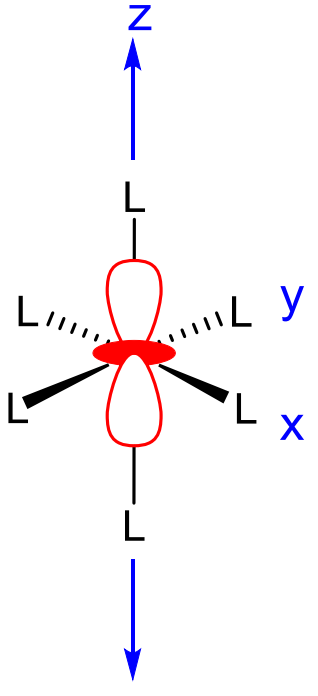
\includegraphics[width=0.5\linewidth]{Imágenes/JTE-z-out-draw.png}
        \caption{}
    \end{subfigure}
    %\hfill % Espacio horizontal entre imágenes
    \begin{subfigure}{0.2\textwidth}
        \centering
        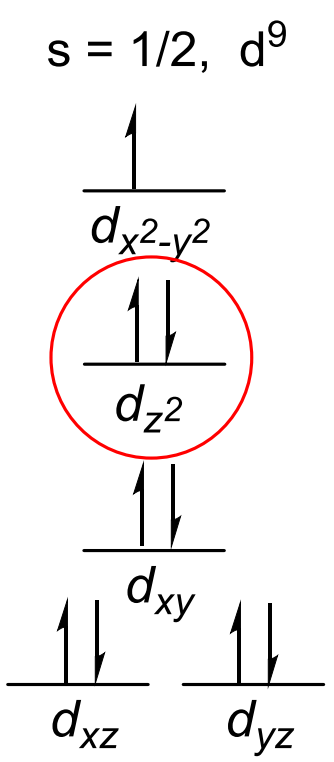
\includegraphics[width=0.5\linewidth]{Imágenes/JTE-z-out-orbitals.png}
        \caption{}
    \end{subfigure}
    
    \vspace{0.5cm} % Espacio vertical entre filas
    
    % Fila inferior: Distorsión z-in (Compresión)
    \begin{subfigure}{0.3\textwidth}
        \centering
        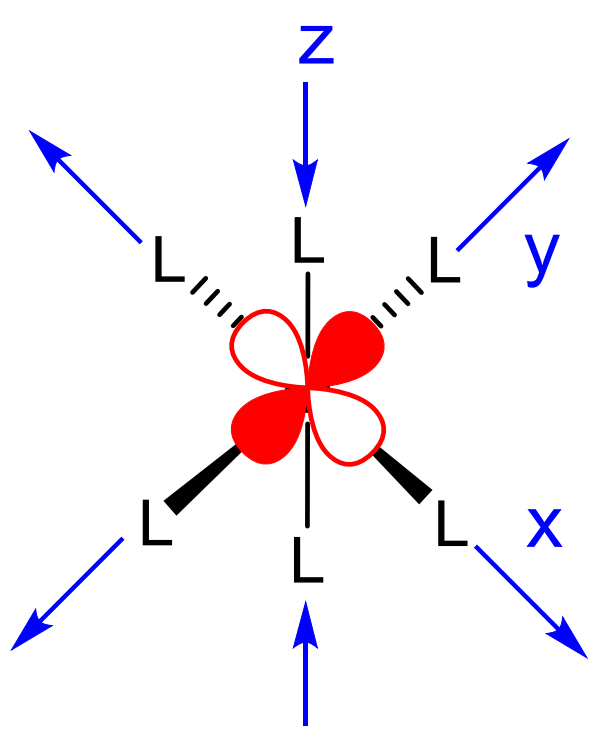
\includegraphics[width=0.5\linewidth]{Imágenes/JTE-z-in-draw.png}
        \caption{}
    \end{subfigure}
    %\hfill % Espacio horizontal entre imágenes
    \begin{subfigure}{0.2\textwidth}
        \centering
        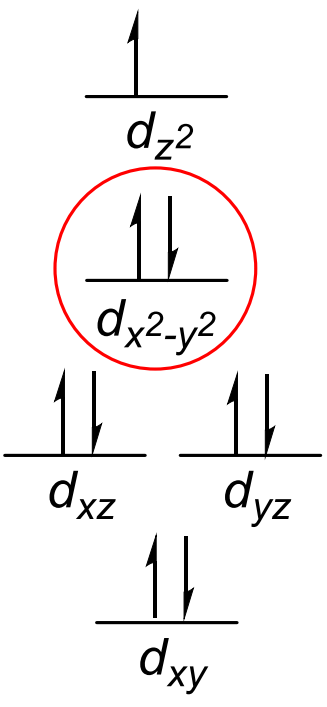
\includegraphics[width=0.5\linewidth]{Imágenes/JTE-z-in-orbitals.png}
        \caption{}
    \end{subfigure}
    
    \caption{Ilustración  del efecto Jahn-Teller de \cite{Cu-2019-01} para un complejo octaédrico del ion Cu(II) con configuración electrónica $d^9$. Arriba se muestra la distorsión por elongación axial (z-out), donde los enlaces axiales se alargan, y su correspondiente desdoblamiento de orbitales. Abajo se presenta la distorsión por compresión axial (z-in), con el acortamiento de los enlaces axiales y su respectivo desdoblamiento energético. La distorsión z-out es la observada más comúnmente en la experimentación .}
    \label{fig:jahn_teller_cu2}
\end{figure}


Aunque la elongación es la geometría más común, estudios teóricos han demostrado que ambas son posibles para el catión \ce{[Cu(OH2)6]^{2+}} \cite{Cu-2019-01}.

El JTE no es un mero detalle, sino la causa directa de la química de coordinación excepcionalmente flexible y dinámica del \ce{Cu^{2+}}. Dota al ion de una plasticidad estructural inusual, permitiéndole adoptar múltiples geometrías (octaédrica distorsionada, piramidal cuadrada, planar cuadrada) con diferencias energéticas muy pequeñas entre ellas. Esta flexibilidad es inherentemente dinámica; en solución, el complejo interconvierte rápidamente entre estas configuraciones. Esto explica la alta labilidad de sus ligandos, cuya tasa de intercambio es órdenes de magnitud superior a la de otros cationes divalentes. La debilidad de los enlaces axiales facilita este rápido intercambio y ha generado un prolongado debate sobre el número de coordinación preferido (4, 5 o 6) del ion en solución.

\section{Hidratación}

\subsection*{Estudios Experimentales}

Históricamente, los estudios experimentales han sido la piedra angular en la comprensión de la solvatación del Cu\textsuperscript{2+}. Las técnicas más utilizadas incluyen:
\begin{itemize}
    \item Difracción de Rayos X y Neutrones
    \item Espectroscopia de Absorción de Rayos X (EXAFS y XANES)
\end{itemize}

Los primeros trabajos de difracción en las décadas de 1970 y 1980 establecieron la idea de una coordinación octaédrica distorsionada (NC=6), con una configuración (4+2) que implicaba cuatro ligandos de agua en posiciones ecuatoriales y dos más distantes en posiciones axiales. Sin embargo, a partir del año 2000, estudios más avanzados, que combinaban técnicas como la difracción de neutrones con dinámica molecular o empleaban análisis de EXAFS y XANES más sofisticados, comenzaron a favorecer un modelo de **coordinación quíntuple (NC=5)** con una geometría de pirámide cuadrada.

Actualmente, existe un consenso experimental sobre las distancias de enlace ecuatoriales ($Cu-O_{eq}$), que se reportan consistentemente en el rango de **1.93--2.00 \AA**. Por el contrario, las distancias axiales ($Cu-O_{ax}$) son más difíciles de medir y presentan una mayor variabilidad, con valores que oscilan entre **2.15 \AA \ y 2.60 \AA**. Investigaciones recientes de alta resolución sugieren incluso la existencia de dos distancias axiales distintas, lo que apunta a un octaedro no centrosimétrico. Algunos estudios que emplean un enfoque multitécnica han llegado a proponer un NC promedio de 4.5, lo que refuerza la idea de una mezcla dinámica de geometrías en solución. La imagen moderna, por tanto, describe una "plasticidad estructural" donde múltiples estados de coordinación coexisten en un equilibrio dinámico.

\subsection*{Estudios Teóricos}

Los estudios computacionales han sido fundamentales para interpretar la evidencia experimental y proporcionar una visión dinámica del proceso de solvatación. Los principales métodos teóricos empleados son:
\begin{itemize}
    \item Teoría del Funcional de la Densidad (DFT)
    \item Dinámica Molecular (MD), tanto clásica como \textit{ab initio} (AIMD)
    \item Métodos híbridos de Mecánica Cuántica/Mecánica Molecular (QM/MM)
\end{itemize}

Las simulaciones teóricas corroboran la naturaleza dinámica del efecto Jahn-Teller, mostrando transformaciones rápidas entre diferentes configuraciones en escalas de tiempo de femtosegundos. Gran parte de los modelos teóricos indican que la geometría de **pirámide cuadrada (NC=5)** es la más estable en solución acuosa, aunque la diferencia de energía con la forma **hexa-coordinada (NC=6)** es muy pequeña ($\sim$1.4 kcal/mol). Esto sugiere que ambas especies pueden coexistir en solución, lo cual está en línea con los hallazgos experimentales más recientes.

Un aporte crucial de los estudios teóricos ha sido resaltar el papel de la segunda capa de solvatación. Se ha demostrado que la formación de enlaces de hidrógeno entre las moléculas de agua de la primera y segunda esfera de hidratación es un factor de estabilización que puede competir energéticamente con la coordinación de una molécula de agua en la posición axial. Las distancias de enlace calculadas concuerdan bien con los datos experimentales, con valores promedio para $Cu-O_{eq}$ de alrededor de **2.00--2.03 \AA** y para $Cu-O_{ax}$ de **2.15--2.30 \AA**. En general, la modelización teórica apoya la visión de un sistema flexible donde coexisten dinámicamente estructuras con NC=5 y NC=6, y descarta una relevancia significativa de la coordinación tetraédrica (NC=4) en el ion Cu\textsuperscript{2+} solvatado en agua.

\section{Solvatación  en Metanol}


Al igual que en el agua, la estructura de solvatación del ion Cu\textsuperscript{2+} en metanol es un área de investigación activa, aunque la cantidad de estudios disponibles es notablemente más escasa. Persiste un debate sobre el número de coordinación (NC) y la geometría predominantes, con diferentes estudios experimentales y teóricos llegando a conclusiones contradictorias. La naturaleza dinámica del ion y la sutil influencia del disolvente complican la obtención de un consenso definitivo. Un resumen detallado de los trabajos más relevantes se encuentra en la Tabla \ref{tab:metanol_corrected}.

\subsection*{Estudios Experimentales}

Las investigaciones experimentales han empleado diversas técnicas espectroscópicas para determinar la estructura local del Cu\textsuperscript{2+} en metanol. Entre los métodos más destacados se encuentran:
\begin{itemize}
    \item Espectroscopia de absorción de rayos X (EXAFS y XANES)
    \item Análisis de modulación de eco de espín de electrones
    \item Estudios de Resonancia Magnética Nuclear (RMN) de Oxígeno-17
\end{itemize}

El panorama experimental se caracteriza por una falta de acuerdo. Mientras que estudios tempranos (Ichikawa y Kevan, 1980) propusieron una coordinación de \textbf{seis (NC=6)}, trabajos posteriores sugirieron que la técnica empleada podría haber sobrestimado las distancias de enlace. Más tarde, estudios de RMN (Helm et al., 1986) observaron una "rápida transición" de isómeros hexacoordinados a conformaciones de \textbf{cinco coordinaciones (NC=5)}, introduciendo la idea de un equilibrio dinámico.

Este debate continúa en estudios más recientes. Por un lado, Zitolo et al. (2012), combinando EXAFS y XANES, concluyeron "inequívocamente" que el Cu\textsuperscript{2+} en metanol adopta una geometría de \textbf{pirámide cuadrada con NC=5}. Por otro lado, un estudio más reciente de Persson et al. (2020) con EXAFS de alta calidad determinó que el mejor modelo de ajuste correspondía a una estructura \textbf{octaédrica distorsionada por Jahn-Teller con NC=6} y carácter no centrosimétrico, contradiciendo directamente la conclusión anterior.

A pesar de la discrepancia en el NC, hay un mayor consenso en las distancias de enlace ecuatoriales ($Cu-O_{eq}$), reportadas consistentemente en el rango de \textbf{1.95--1.98 \AA}. Las distancias axiales ($Cu-O_{ax}$), sin embargo, varían más, con valores reportados de \textbf{2.23 \AA} para el modelo de NC=5 y dos distancias distintas de aproximadamente \textbf{2.20 \AA \ y 2.34 \AA} para el modelo de NC=6.

\subsection*{Estudios Teóricos}

Los métodos computacionales han sido cruciales para explorar el complejo panorama energético de la solvatación del Cu\textsuperscript{2+} en metanol. Las principales técnicas utilizadas incluyen:
\begin{itemize}
    \item Métodos \textit{ab initio} como MP2
    \item Teoría del Funcional de la Densidad (DFT), en particular con el funcional M06-2X
    \item Modelos de disolvente continuo implícito (IEF-PCM)
\end{itemize}

Los estudios teóricos, principalmente los trabajos exhaustivos de Da-yang et al., han demostrado que el NC más estable depende fuertemente de las condiciones del modelo, como el tamaño del clúster de solvente (n), la temperatura y el entorno (fase gaseosa vs. disolvente implícito).

En la \textbf{fase gaseosa}, los cálculos muestran una competencia entre diferentes números de coordinación. El método MP2 tiende a favorecer isómeros \textbf{tetra- y pentacoordinados}, mientras que el método DFT (M06-2X) favorece a los \textbf{penta- y hexacoordinados}. Para clústeres pequeños (n=1-5), las coordinaciones más bajas son las más estables, pero a medida que aumenta el tamaño, las estructuras de mayor NC ganan relevancia.

La inclusión de un \textbf{modelo de disolvente implícito} (IEF-PCM) tiene un "impacto discernible" y cambia drásticamente el panorama. En este entorno, se observa una clara preferencia por los números de coordinación más altos, desfavoreciendo a las estructuras de NC=4. Para clústeres de mayor tamaño (n=7-10), las estructuras \textbf{hexacoordinadas (NC=6)} dominan "exclusivamente" la población a cualquier temperatura. Este hallazgo subraya la importancia crítica del efecto del medio dieléctrico para estabilizar geometrías más compactas y con mayor número de coordinación.

Las distancias de enlace calculadas teóricamente muestran una "excelente concordancia" con los datos experimentales, con valores de $Cu-O_{eq}$ que oscilan entre \textbf{1.94--2.02 \AA} y de $Cu-O_{ax}$ entre \textbf{2.15--2.27 \AA}. Los cálculos también revelan que el disolvente alarga los enlaces dativos axiales en las estructuras pentacoordinadas en comparación con la fase gaseosa.



\section{Justificación y Enfoque Metodológico}

Históricamente, los métodos experimentales como la difracción de rayos X y neutrones o las espectroscopias EXAFS y XANES han sido cruciales para sondear estos sistemas. Sin embargo, a pesar de su capacidad para medir distancias de enlace con precisión, estos métodos enfrentan limitaciones significativas. A menudo existe una considerable controversia y ambigüedad en la determinación del número de coordinación (NC) y la geometría, y resulta técnicamente difícil distinguir entre estructuras con energías muy similares, como las de coordinación cuádruple, quíntuple y séxtuple, que pueden coexistir en solución.

Frente a estas limitaciones, los métodos teóricos y las simulaciones computacionales emergen como una herramienta indispensable y complementaria. Enfoques como la Dinámica Molecular (MD) basada en la Teoría del Funcional de la Densidad (DFT) permiten superar las desventajas experimentales al proporcionar una visión detallada a nivel atómico. Estos métodos posibilitan la exploración de superficies de energía potencial, la caracterización de efectos dinámicos como la inversión del eje de Jahn-Teller en escalas de tiempo de picosegundos, y el estudio de interacciones complejas como la transferencia de carga y los enlaces de hidrógeno, que son difíciles de aislar experimentalmente. Si bien los métodos teóricos no están exentos de desventajas, como el alto costo computacional y una fuerte sensibilidad a la elección del funcional y la base de conjunto, su capacidad para modelar la dinámica y la coexistencia de múltiples estados los convierte en una opción poderosa para resolver las controversias existentes.

El presente trabajo de tesis aprovecha las ventajas de los métodos teóricos para abordar dos frentes. Primero, se enfoca en la solvatación del Cu\textsuperscript{2+} en metanol, un área donde la información experimental y teórica es notablemente más escasa en comparación con el agua. Este vacío de conocimiento representa un área de oportunidad significativa. Por ello, este trabajo presenta por primera vez en la literatura un estudio teórico exhaustivo sobre la estructura y dinámica de los clústeres de Cu\textsuperscript{2+}(MeOH)\textsubscript{n} utilizando DFT. Segundo, se reexamina el caso del agua. Aunque es un sistema mucho más estudiado, la controversia sobre la predominancia de una coordinación quíntuple o séxtuple persiste. El enfoque teórico permite analizar la coexistencia dinámica de estas especies, ofreciendo una perspectiva que las mediciones experimentales, a menudo promediadas en el tiempo, no pueden capturar completamente.

Para llevar a cabo estos estudios, se ha seleccionado el funcional \textbf{M06-2X}. Esta elección se justifica brevemente aquí, y se detallará a profundidad en capítulos posteriores. El M06-2X se presenta como una alternativa computacionalmente eficiente a métodos \textit{ab initio} más costosos como el MP2, y ha demostrado una excelente concordancia con datos experimentales y teóricos para la descripción de los clústeres de Cu\textsuperscript{2+} en metanol, reproduciendo con precisión las distancias de enlace y las reglas de estabilidad.

En los siguientes capítulos se expondrá el marco teórico detallado de la Dinámica Molecular y la Teoría del Funcional de la Densidad, explicando la naturaleza del funcional M06-2X. Posteriormente, se presentará la metodología computacional empleada para la construcción y simulación de los sistemas en ambos disolventes. Finalmente, se realizará un análisis exhaustivo de los resultados y se presentarán las conclusiones derivadas de este estudio computacional.

        \chapter{Dinámica molecular}

\section{Dinámica molecular clásica}

La dinámica molecular (DM) clásica modela un sistema de átomos y moléculas resolviendo numéricamente las ecuaciones de movimiento de Newton. En este enfoque, los átomos son tratados como partículas clásicas que interactúan a través de un conjunto de funciones de energía potencial, conocido como campo de fuerza (\textit{force field}). Este método es computacionalmente eficiente y puede aplicarse a sistemas muy grandes, de hasta millones de átomos, y a escalas de tiempo de nanosegundos o más.

\subsection{QM/MM}

Para sistemas donde ocurren fenómenos cuánticos, como la ruptura o formación de enlaces, en una región específica de un sistema molecular grande, el enfoque híbrido de Mecánica Cuántica/Mecánica Molecular (QM/MM) es particularmente útil. El concepto central del método QM/MM es dividir el sistema en dos regiones. La parte donde los efectos electrónicos son críticos, como el ion \ce{Cu^{2+}} y su primera esfera de solvatación, se trata con métodos de mecánica cuántica (QM) de alta precisión. El entorno circundante, como el resto de las moléculas de disolvente, se describe mediante un campo de fuerza de mecánica molecular (MM), que es computacionalmente menos demandante.

La interacción entre ambas regiones es un aspecto clave. En el esquema más común, llamado \textbf{inclusión electrónica} (\textit{electronic embedding}), las cargas parciales de los átomos de la región MM se incorporan al Hamiltoniano de la región QM, permitiendo que la región cuántica se polarice por su entorno clásico.

Los campos de fuerza utilizados en la parte MM se basan en un modelo de "esferas y resortes", donde la energía total es una suma de términos que describen las interacciones atómicas. Para el estudio de la solvatación del ion cúprico se han empleado diversas aproximaciones:

\begin{itemize}
    \item \textbf{Energía de enlace y ángulo:} Términos que describen la energía asociada a la compresión o estiramiento de un enlace covalente (\textit{stretch}) y a la flexión del ángulo entre tres átomos (\textit{bend}).
    
    \item \textbf{Energía torsional:} Representa la energía relacionada con la rotación alrededor de un enlace, definida por un ángulo diedro.
    
    \item \textbf{Interacciones no enlazadas:} Modelan las interacciones entre átomos que no están directamente enlazados. Se componen de un término de van der Waals, que describe la repulsión y la atracción por dispersión (a menudo con un potencial de Lennard-Jones), y un término electrostático, que describe las interacciones de largo alcance basadas en cargas atómicas parciales. En simulaciones clásicas del ion \ce{Cu^{2+}}, este se ha descrito a menudo como una simple esfera de van der Waals, con parámetros de Lennard-Jones ajustados a partir de cálculos \textit{ab initio}. Se han utilizado campos de fuerza de todos los átomos como OPLS y modelos de agua no polarizables como TIP3P.
    
    \item \textbf{Campos de fuerza polarizables:} Para superar las limitaciones de los campos de fuerza clásicos, se han desarrollado modelos que tienen en cuenta explícitamente la polarización electrónica. Estos modelos permiten que las polarizabilidades atómicas o moleculares generen dipolos inducidos en respuesta al campo eléctrico del soluto, ofreciendo una descripción más precisa de las interacciones. Para el ion \ce{Cu(II)}, se ha aplicado el campo de fuerza polarizable AMOEBA y se han utilizado modelos de agua avanzados como SWM4-DP.
    
    \item \textbf{Métodos QM/MM específicos:} Se han realizado numerosas simulaciones de Dinámica Molecular QM/MM para investigar la hidratación del \ce{Cu^{2+}} y su efecto Jahn-Teller en solución. Se han empleado metodologías como el Campo de Carga Mecánico Cuántico (QMCF) y el método secuencial QM/MM, donde se realizan cálculos QM sobre configuraciones seleccionadas de una simulación MM.
\end{itemize}

\subsection{Limitaciones}
A pesar de su utilidad, los métodos de DM clásica y QM/MM presentan limitaciones importantes, especialmente para un ion tan complejo como el \ce{Cu^{2+}}. Una de las principales deficiencias de los campos de fuerza clásicos es su incapacidad para describir correctamente la distorsión de Jahn-Teller, ya que esta es de origen puramente electrónico. Además, estos modelos a menudo ignoran efectos cruciales de muchos cuerpos, la polarización y la transferencia de carga entre el ion y las moléculas de disolvente. El uso de cargas parciales fijas, común en la mayoría de los campos de fuerza, puede ser inadecuado para un ion altamente polarizante como el \ce{Cu^{2+}}, lo que podría conducir a resultados incorrectos.

Por su parte, los métodos QM/MM, aunque superiores, no son "cajas negras". No existe una forma única de decidir cómo dividir el sistema entre las regiones QM y MM, y la manera de "unir" ambas regiones no es única, lo que los convierte en métodos que aún se consideran "experimentales" en cierto grado.

\section{Dinámica molecular ab initio}

La dinámica molecular \textit{ab initio} (AIMD) supera muchas de las limitaciones de los métodos clásicos. En este enfoque, las fuerzas que actúan sobre los núcleos se calculan "al vuelo" en cada paso de la simulación a partir de un cálculo de estructura electrónica, generalmente basado en la Teoría del Funcional de la Densidad (DFT). Esto permite modelar explícitamente la polarización electrónica y los eventos reactivos como la ruptura y formación de enlaces.

\subsection{Dinámica molecular de Car-Parrinelo}

La Dinámica Molecular de Car-Parrinelo (CPMD), desarrollada en 1985, es un método de AIMD que trata simultáneamente los grados de libertad nucleares y electrónicos. Su idea fundamental es introducir una dinámica ficticia para los parámetros de la función de onda (los orbitales), a los que se les asigna una masa ficticia. De esta manera, los orbitales evolucionan en el tiempo junto con las posiciones nucleares dentro de un formalismo de Lagrange extendido.

La gran ventaja de CPMD es que elimina la necesidad de converger completamente la función de onda en cada paso de tiempo, un proceso que es muy costoso en otros métodos de AIMD. El método funciona bajo la condición de que se mantenga una separación adiabática entre la dinámica nuclear, que es más lenta, y la dinámica electrónica ficticia, que es más rápida.

A pesar de ser un método robusto y citado en muchos trabajos de referencia sobre la solvatación del \ce{Cu^{2+}} , puede enfrentar dificultades en sistemas con una brecha energética (\textit{gap}) pequeña o nula entre los estados electrónicos, donde la condición de adiabaticidad podría romperse. Estudios teóricos previos sobre el sistema acuoso del \ce{Cu^{2+}} han empleado CPMD con funcionales de tipo GGA, como BLYP y PBE. Sin embargo, se ha demostrado que funcionales como BLYP pueden subestimar la afinidad de enlace de la sexta molécula de agua al ion y sobrestimar la estabilidad de las estructuras de baja coordinación en comparación con métodos de mayor nivel, lo que limita su capacidad para describir con precisión la compleja estructura electrónica del cobre(II).

\section{Dinámica Molecular de Bohr-Oppenheimer}

        %
\chapter{Teoría de los Funcionales de la Densidad}
\label{chap:dft}

La resolución de la ecuación de Schrödinger para sistemas polielectrónicos es uno de los desafíos centrales de la química cuántica \cite[68]{szabo1996modern}. Dado que una solución analítica exacta es inviable para sistemas de más de un electrón, se han desarrollado métodos aproximados para obtener soluciones numéricas de alta precisión. Históricamente, estos métodos se han basado en la aproximación de la función de onda. Sin embargo, en las últimas décadas, la Teoría de los Funcionales de la Densidad (DFT) ha emergido como una alternativa robusta y computacionalmente eficiente, posicionándose como una de las herramientas más utilizadas en la química computacional moderna \cite[6]{koch2015chemist}.

Este capítulo establece el marco teórico que fundamenta los cálculos de DFT. Se parte de las aproximaciones fundamentales de la química cuántica, como la aproximación de Born-Oppenheimer, para luego introducir el método de Hartree-Fock y sus limitaciones inherentes. Posteriormente, se presenta la DFT como una solución elegante a estos desafíos, detallando sus pilares teóricos —los teoremas de Hohenberg-Kohn— y su implementación práctica a través del formalismo de Kohn-Sham. Finalmente, se discute la jerarquía de los funcionales de intercambio y correlación, culminando con una descripción del funcional M06-2X, empleado en este trabajo de tesis.

\section{Fundamentos: De la Ecuación de Schrödinger a Hartree-Fock}

\subsection{La Aproximación de Born-Oppenheimer}
La aproximación de Born-Oppenheimer es un pilar fundamental en la química cuántica que permite desacoplar el movimiento de los electrones y los núcleos \cite[p. 58]{szabo1996modern}. Se fundamenta en la gran diferencia de masa entre los núcleos y los electrones; al ser los núcleos mucho más pesados, se mueven considerablemente más lento. Por lo tanto, es posible considerar que los electrones se mueven en un campo electrostático generado por núcleos en posiciones fijas.

Dentro de esta aproximación, el término de energía cinética de los núcleos en el Hamiltoniano total se desprecia, y la repulsión internuclear se considera una constante para una configuración nuclear dada \cite[p. 58]{szabo1996modern}. Esto simplifica enormemente el problema, permitiendo resolver la ecuación de Schrödinger exclusivamente para los electrones, conocida como la ecuación de Schrödinger electrónica:
$$ \hat{H}_{\text{elec}} \Psi_{\text{elec}} = E_{\text{elec}} \Psi_{\text{elec}} $$
donde el Hamiltoniano electrónico, $\hat{H}_{\text{elec}}$, describe el movimiento de $N$ electrones en el campo de $M$ núcleos fijos y se compone de la energía cinética de los electrones, la atracción electrón-núcleo y la repulsión electrón-electrón. Aunque esta aproximación introduce errores pequeños, estos son generalmente insignificantes para la mayoría de los sistemas, excepto para aquellos con núcleos muy ligeros como el hidrógeno, donde pueden ser necesarias correcciones \cite[p. 107]{jensen2017introduction}.

\subsection{La Aproximación de Hartree-Fock}
La aproximación de Hartree-Fock (HF), también conocida como la aproximación de orbitales moleculares, es un concepto central en la química y a menudo constituye el punto de partida para métodos más sofisticados que incluyen la correlación electrónica \cite[p. 123]{szabo1996modern}. En este modelo, se asume que la función de onda de un sistema de $N$ electrones puede ser aproximada por un único determinante de Slater, construido a partir de un conjunto de $N$ espín-orbitales.
$$ \Psi_{\text{HF}} = \frac{1}{\sqrt{N!}} \det[\chi_1(x_1) \chi_2(x_2) \dots \chi_N(x_N)] $$
Este enfoque considera que cada electrón se mueve de forma independiente en un campo promedio generado por los demás electrones, en lugar de interactuar instantáneamente con cada uno de ellos. Las ecuaciones de Hartree-Fock se resuelven de manera iterativa mediante el procedimiento de campo autoconsistente (SCF, por sus siglas en inglés), hasta que los orbitales y el campo promedio que generan ya no cambian significativamente entre iteraciones \cite[p. 69]{szabo1996modern}.

Sin embargo, la aproximación de HF tiene limitaciones importantes. Al promediar las interacciones electrón-electrón, ignora la correlación en el movimiento de los electrones. La diferencia entre la energía exacta no relativista y la energía obtenida en el límite de Hartree-Fock se define como la \textbf{energía de correlación} \cite[p. 246]{szabo1996modern}. Esta omisión causa que el método HF sea cualitativamente incorrecto para describir procesos como la disociación de moléculas en fragmentos de capa abierta (e.g., H$_2$ $\rightarrow$ 2H$\cdot$) \cite[p. 246]{szabo1996modern}.

\subsection{Conjuntos de Bases (Basis Sets)}
En la práctica computacional, los orbitales moleculares se describen matemáticamente como una combinación lineal de un conjunto de funciones predefinidas, conocidas como \textbf{conjunto de bases} (o *basis set*). Un conjunto de bases es, por tanto, una descripción matemática de los orbitales de un sistema que se utiliza para realizar cálculos teóricos aproximados \cite[131]{ramachandran2008computational}. La calidad de un cálculo depende críticamente de la flexibilidad y completitud de este conjunto de funciones.
$$ \psi_i = \sum_{\mu=1}^{k} c_{\mu i} \phi_{\mu} $$
donde $\psi_i$ es el orbital molecular, $\phi_{\mu}$ son las funciones de base y $c_{\mu i}$ son los coeficientes de la combinación lineal. Comúnmente se utilizan funciones de tipo Gaussiano (GTOs) en lugar de las de tipo Slater (STOs) por su eficiencia computacional en el cálculo de integrales. Existen jerarquías de conjuntos de bases, como los desarrollados por Pople (e.g., 6-31G*, 6-311+G**), que ofrecen un compromiso entre precisión y costo computacional al mejorar la descripción de la valencia y añadir funciones de polarización y difusas \cite[195]{szabo1996modern}, \cite[140]{ramachandran2008computational}.

\section{La Revolución de DFT: El Paradigma de la Densidad}

\subsection{La Densidad Electrónica y la Densidad de Pares}
La Teoría de los Funcionales de la Densidad (DFT) se basa en el uso de la \textbf{densidad electrónica}, $\rho(\mathbf{r})$, como la variable fundamental, en lugar de la compleja función de onda de N-electrones \cite[187]{ramachandran2008computational}. La densidad electrónica es una función de solo tres variables espaciales $(x, y, z)$ y determina la probabilidad de encontrar cualquiera de los $N$ electrones en un elemento de volumen $d\mathbf{r}$ \cite[36]{koch2015chemist}.
$$ \rho(\mathbf{r}_1) = N \int \dots \int |\Psi(x_1, x_2, \dots, x_N)|^2 \, ds_1 \, dx_2 \dots dx_N $$
A diferencia de la función de onda, $\rho(\mathbf{r})$ es una cantidad observable experimentalmente, por ejemplo, mediante difracción de rayos X. Su complejidad no aumenta con el número de electrones, lo que la convierte en una variable mucho más manejable \cite[p. 253]{jensen2017introduction}.

Un concepto relacionado es la \textbf{densidad de pares}, $\rho_2(\mathbf{r}_1, \mathbf{r}_2)$, que describe la probabilidad de encontrar simultáneamente un par de electrones en dos elementos de volumen, $d\mathbf{r}_1$ y $d\mathbf{r}_2$. Esta cantidad es de suma importancia, ya que contiene toda la información sobre la correlación electrónica, es decir, cómo el movimiento de un electrón afecta al de otro \cite[188]{ramachandran2008computational}, \cite[38]{koch2015chemist}.

\subsection{Los Teoremas de Hohenberg-Kohn}
La base formal de la DFT reside en dos teoremas fundamentales demostrados por Pierre Hohenberg y Walter Kohn en 1964.

El \textbf{primer teorema de Hohenberg-Kohn} establece que el potencial externo, $V_{\text{ext}}(\mathbf{r})$, y por lo tanto el Hamiltoniano total, está determinado unívocamente (salvo una constante aditiva) por la densidad electrónica del estado fundamental, $\rho_0(\mathbf{r})$ \cite[50]{koch2015chemist}. Dado que el Hamiltoniano define todas las propiedades del sistema, se concluye que la energía del estado fundamental y todas las demás propiedades son funcionales únicos de la densidad del estado fundamental. En resumen:
$$ \rho_0(\mathbf{r}) \implies \hat{H} \implies \Psi_0 \implies E_0 $$
Esto establece una correspondencia uno a uno entre la densidad electrónica de un sistema y su energía \cite[253]{jensen2017introduction}.

El \textbf{segundo teorema de Hohenberg-Kohn} introduce un principio variacional para la densidad. Afirma que el funcional que proporciona la energía del estado fundamental, $E_0$, a partir de la densidad, $E[\rho]$, alcanza su valor mínimo si y solo si la densidad de entrada es la verdadera densidad del estado fundamental, $\rho_0$ \cite[53]{koch2015chemist}. Para cualquier densidad de prueba, $\tilde{\rho}(\mathbf{r})$, que sea físicamente aceptable, la energía calculada será un límite superior a la energía verdadera del estado fundamental:
$$ E_0 \le E[\tilde{\rho}] $$
Esto proporciona una ruta para encontrar la densidad y la energía del estado fundamental: minimizar el funcional de la energía con respecto a la densidad \cite[53]{koch2015chemist}. El problema principal, sin embargo, es que la forma exacta del funcional universal de la energía, $F_{HK}[\rho]$, no se conoce.

\section{La Implementación Práctica: El Método de Kohn-Sham}
En 1965, Walter Kohn y Lu Jeu Sham propusieron un método ingenioso para aplicar los teoremas de Hohenberg-Kohn de manera práctica. La idea central es reemplazar el difícil problema de modelar el sistema real de electrones que interactúan, por un sistema ficticio de electrones \textbf{no interactuantes} que, por definición, produce la misma densidad electrónica que el sistema real \cite[58]{koch2015chemist}.

La energía cinética de este sistema de referencia no interactuante, $T_s[\rho]$, puede calcularse de manera exacta a partir de sus orbitales, los llamados \textbf{orbitales de Kohn-Sham (KS)}. La energía total del sistema real se reescribe como:
$$ E_{KS}[\rho] = T_s[\rho] + J[\rho] + E_{Ne}[\rho] + E_{XC}[\rho] $$
donde $J[\rho]$ es la energía de repulsión de Coulomb clásica (interacción de la densidad consigo misma) y $E_{Ne}[\rho]$ es la energía de atracción núcleo-electrón. El término clave es el \textbf{funcional de intercambio y correlación}, $E_{XC}[\rho]$. Este funcional agrupa todas las complejidades cuánticas del problema:
\begin{enumerate}
    \item La diferencia entre la energía cinética real y la del sistema no interactuante ($T[\rho] - T_s[\rho]$).
    \item Todos los efectos no clásicos de la repulsión electrón-electrón, incluyendo el intercambio y la correlación \cite[194]{ramachandran2008computational}.
\end{enumerate}
El gran logro del método de Kohn-Sham es que la mayor parte de la energía total se calcula de forma exacta o casi exacta, dejando solo una porción relativamente pequeña, $E_{XC}[\rho]$, que debe ser aproximada \cite[58]{koch2015chemist}.

Los orbitales de KS se obtienen resolviendo un conjunto de ecuaciones de un solo electrón, similares a las de Hartree-Fock, conocidas como las \textbf{ecuaciones de Kohn-Sham}:
$$ \left( -\frac{1}{2}\nabla^2 + V_{\text{eff}}(\mathbf{r}) \right) \phi_i(\mathbf{r}) = \varepsilon_i \phi_i(\mathbf{r}) $$
donde el potencial efectivo, $V_{\text{eff}}$, incluye el potencial externo, el potencial de Coulomb clásico y el potencial de intercambio-correlación, $V_{XC}(\mathbf{r}) = \frac{\delta E_{XC}[\rho]}{\delta \rho(\mathbf{r})}$. Estas ecuaciones se resuelven de forma autoconsistente.

\section{La Jerarquía de Funcionales: "La Escalera de Jacob"}
Dado que la forma exacta de $E_{XC}[\rho]$ es desconocida, el desarrollo de la DFT se ha centrado en la creación de aproximaciones cada vez más precisas. Esta búsqueda ha dado lugar a una jerarquía de funcionales, a menudo denominada "La Escalera de Jacob", donde cada peldaño representa un mayor nivel de sofisticación y, generalmente, de precisión.

\subsection{Aproximación de Densidad Local (LDA)}
Es el peldaño más simple. La Aproximación de Densidad Local (LDA) asume que la densidad en cualquier punto $\mathbf{r}$ se comporta como un gas de electrones homogéneo (o uniforme) con esa misma densidad $\rho(\mathbf{r})$ \cite[90]{koch2015chemist}.
$$ E_{XC}^{\text{LDA}}[\rho] = \int \rho(\mathbf{r}) \epsilon_{xc}^{\text{unif}}(\rho(\mathbf{r})) d\mathbf{r} $$
donde $\epsilon_{xc}^{\text{unif}}$ es la energía de intercambio-correlación por partícula de un gas de electrones uniforme. A pesar de su simplicidad, la LDA proporciona resultados razonables para propiedades estructurales, pero tiende a sobreestimar significativamente las energías de enlace (problema de "overbinding") \cite[91]{koch2015chemist}.

\subsection{Aproximación del Gradiente Generalizado (GGA)}
Para mejorar la LDA, la Aproximación del Gradiente Generalizado (GGA) no solo considera la densidad en un punto, $\rho(\mathbf{r})$, sino también su gradiente, $\nabla\rho(\mathbf{r})$ \cite[92]{koch2015chemist}. Esto permite que el funcional tenga en cuenta la no homogeneidad de la densidad electrónica en moléculas y sólidos.
$$ E_{XC}^{\text{GGA}}[\rho] = \int f(\rho(\mathbf{r}), \nabla\rho(\mathbf{r})) d\mathbf{r} $$
Funcionales populares como B88 para el intercambio (de Becke) y LYP para la correlación (de Lee, Yang y Parr) pertenecen a esta categoría. Los funcionales GGA, como BLYP o PBE, representan una mejora sustancial sobre la LDA para el cálculo de energías de enlace y otras propiedades químicas \cite[p. 9]{MD-2002-01}.

\subsection{Funcionales meta-GGA}
El siguiente peldaño en la jerarquía introduce una dependencia adicional de la \textbf{densidad de energía cinética} de los orbitales de Kohn-Sham, $\tau(\mathbf{r})$:
$$ \tau(\mathbf{r}) = \frac{1}{2} \sum_i^{occ} |\nabla\phi_i(\mathbf{r})|^2 $$
Los funcionales meta-GGA utilizan $\rho$, $\nabla\rho$ y $\tau$ para construir el funcional de intercambio-correlación.
$$ E_{XC}^{\text{meta-GGA}}[\rho] = \int g(\rho(\mathbf{r}), \nabla\rho(\mathbf{r}), \tau(\mathbf{r})) d\mathbf{r} $$
Esta información adicional permite a los funcionales meta-GGA satisfacer más restricciones exactas y, en muchos casos, ofrecer una mayor precisión que los GGA, especialmente para barreras de reacción y sistemas metálicos \cite[p. 9]{MD-2002-01}.

\subsection{Funcionales Híbridos}
Los funcionales híbridos, propuestos por Becke, representan un avance conceptual significativo. Mezclan una porción de la energía de intercambio "exacta" calculada al estilo de Hartree-Fock con la energía de intercambio y correlación proveniente de un funcional GGA o meta-GGA \cite[273]{jensen2017introduction}. La justificación teórica se basa en el "teorema de la conexión adiabática". La forma general es:
$$ E_{XC}^{\text{híbrido}} = a E_X^{\text{HF}} + (1-a) E_X^{\text{DFT}} + E_C^{\text{DFT}} $$
donde $a$ es un parámetro que determina el porcentaje de intercambio exacto. El funcional B3LYP es el ejemplo más famoso y combina el intercambio de Becke (B88), la correlación de LYP y un 20\% de intercambio exacto de HF. Los funcionales híbridos suelen ofrecer una precisión muy alta para una amplia gama de propiedades termoquímicas y cinéticas en química del grupo principal \cite[99]{koch2015chemist}.

\section{Justificación del Método: El Funcional M06-2X}
El funcional M06-2X, desarrollado por el grupo de Truhlar en la Universidad de Minnesota, pertenece a la familia de los funcionales \textbf{híbridos meta-GGA} \cite[1]{DFT-2008-01}. Fue diseñado específicamente para ofrecer un alto rendimiento en aplicaciones de la química del grupo principal.

El nombre "M06-2X" indica que es un miembro de la suite de funcionales M06 y que contiene una "doble" cantidad (2X) de intercambio no local (Hartree-Fock), con un 54\% de intercambio exacto. Esta alta no-localidad lo hace particularmente adecuado para el estudio de:
\begin{itemize}
    \item Termoquímica del grupo principal.
    \item Cinética química (cálculo de barreras de reacción).
    \item \textbf{Interacciones no covalentes}, como puentes de hidrógeno, interacciones de apilamiento $\pi-\pi$ y fuerzas de dispersión \cite[2]{Me-2025-01}.
\end{itemize}
El M06-2X es un funcional altamente parametrizado, optimizado contra extensas bases de datos de propiedades energéticas para maximizar su precisión en estas áreas \cite[3, 24]{DFT-2008-01}. Su buen desempeño demostrado en la descripción de sistemas moleculares con puentes de hidrógeno lo convierte en una elección robusta para el estudio de los sistemas solvatados que se abordan en esta tesis \cite[2]{Me-2025-01}.


        
\chapter{Anexos}

\begin{sidewaystable}
    \centering
    \caption{Síntesis de Estudios sobre la Solvatación del Ion Cu$^{2+}$ en Agua}
    \label{tab:full}
    {\scriptsize % Abre el entorno para letra pequeña
    
    % --- Tabla Experimental ---
    \textbf{Estudios Experimentales}
    \vspace{2mm} % Un pequeño espacio vertical
    
    \begin{tabular}{@{}lllll@{}}
    \toprule
    \textbf{Referencia (Año)} & \textbf{Técnica} & \textbf{NC (Número de Coordinación)} & \textbf{Distancia Cu-O$_{eq}$ (\AA)} & \textbf{Distancia Cu-O$_{ax}$ (\AA)} \\
    \midrule
    Neilson et al. (1981)   & Difracción de neutrones & 6 $\pm$ 1                              & 1.97 $\pm$ 0.02                      & 2.60 $\pm$ 0.02                                 \\
    Sham et al. (1981)      & EXAFS                   & 4 + 2 (6-coordinado)                   & 1.96                                 & 2.60                                            \\
    Salmon et al. (1988)    & Difracción de neutrones & 4 + 2 (6-coordinado)                   & 1.96 $\pm$ 0.03                      & $\geq$ 2.21 (citado como 2.60)                  \\
    Pasquarello et al. (2001) & Difracción de neutrones y MD & 5-coordinado                           & ~1.95-2.0                            & -                                               \\
    Benfatto et al. (2002)  & EXAFS y XANES           & 5-coordinado (o 6-coordinado)          & 1.961 (para 6-coord)                 & 2.36 (para 6-coord)                             \\
    Frank et al. (2005)     & MXAN y XAS              & Principalmente 5-coordinado          & 1.95 - 1.98 $\pm$ 0.03               & 2.35 $\pm$ 0.05                                 \\
    Amira et al. (2005)     & CPMD                    & 5-coordinado                           & 2.00                                 & 2.45                                            \\
    Smirnov y Trostin (2009)& Revisión                & 6-coordinado                           & 1.96 $\pm$ 0.04                      & 2.40 $\pm$ 0.10                                 \\
    Bowron et al. (2013)    & Multi-técnica           & 4.5 $\pm$ 0.6 (promedio)               & -                                    & -                                               \\
    Frank et al. (2015)     & XAS (alta resolución)   & 5-coordinado (dominante)               & 1.95 - 1.97                          & 2.21 (5-coord), 2.19 y 2.33 (6-coord)           \\
    Frank et al. (2018)     & XAS y MXAN              & 6-coord (55\%) y 5-coord (43\%)        & 1.95 $\pm$ 0.01                      & 2.14 $\pm$ 0.06 y 2.28 $\pm$ 0.05 ("split axial") \\
    Persson et al. (2020)   & EXAFS                   & 6-coordinado (no centrosimétrico)      & 1.956 $\pm$ 0.003                    & 2.14 $\pm$ 0.02 y 2.32 $\pm$ 0.02 ("split axial") \\
    \bottomrule
    \end{tabular}

    \vspace{8mm} % Espacio mayor entre las dos tablas

    % --- Tabla Teórica ---
    \textbf{Estudios Teóricos}
    \vspace{2mm} % Un pequeño espacio vertical

    \begin{tabular}{@{}lllll@{}}
    \toprule
    \textbf{Referencia (Año)} & \textbf{Técnica} & \textbf{NC (Número de Coordinación)} & \textbf{Distancia Cu-O$_{eq}$ (\AA)} & \textbf{Distancia Cu-O$_{ax}$ (\AA)} \\
    \midrule
    Bérces et al. (1999)      & DFT y MD                & 4                                      & -                                    & -                                          \\
    Burda et al. (2004)       & DFT                     & 5 y 6-coordinados estables             & ~1.95-1.97 (5-coord), 1.956 (6-coord)  & 2.170 (5-coord), 2.281 (6-coord)           \\
    Pavelka y Burda (2005)    & DFT                     & 4 y 6-coordinados                      & 1.96 (4-coord), 1.98 (6-coord)       & 2.24 (6-coord)                             \\
    de Almeida et al. (2007)  & DFT (B3LYP)             & 6-coordinado (D2h)                     & 1.968 y 2.047 ("split")              & 2.296                                      \\
    Sukrat y Parasuk (2007)   & HF, MP2, B3LYP          & 5-coordinado (más estable)             & (~1.95)                              & < 2.29                                     \\
    Bryantsev et al. (2008)   & DFT y COSMO             & 5-coordinado (más estable en agua)     & 2.001                                & 2.273                                      \\
    O'Brien y Williams (2008) & Computacional (B3LYP)   & Consistente con 4 (contrib. 5 y 6)     & -                                    & -                                          \\
    Bryantsev et al. (2009)   & DFT y COSMO             & 5-coordinado (más estable)             & 2.001                                & 2.272                                      \\
    Rios-Font et al. (2010)   & DFT                     & 4 o 5-coordinados                      & -                                    & -                                          \\
    Liu et al. (2010)         & MD ab initio            & 5 y 6-coordinados (coexistencia)       & -                                    & -                                          \\
    Gómez-Salces et al. (2012) & Revisión y QM/MM       & 5-coordinación favorecida              & 2.03                                 & 2.15 y 2.30 (no centrosimétricos)          \\
    Galván-García et al. (2017) & DFT                   & Coexistencia de 4, 5, y 6              & 2.047-2.049 (6-coord, MP2)           & 2.215 (6-coord, MP2)                       \\
    Monjaraz-Rodríguez et al. (2018) & DFT              & 5 (domina) y 6                         & ~2.0                                 & hasta 2.5                                  \\
    Suzuki et al. (2019)      & 3D-RISM-SCF             & 5-6 (intercambiables)                  & 1.97-2.00 (Ci), 1.96-2.04 (D2h)      & 2.28 (Ci), 2.25 (D2h)                      \\
    Christensen y Steele (2023) & Química cuántica ab initio & Coexistencia de 4, 5, y 6       & -                                    & -                                          \\
    Da-yang et al. (2024)     & MP2/IEF-PCM             & 4, 5, y 6 (para n=10)                  & 1.99 (5-coord), 2.01 (6-coord)       & 2.19 (5-coord), 2.26 (6-coord)             \\
    \bottomrule
    \end{tabular}
    
    } % Cierra el entorno de letra pequeña
\end{sidewaystable}




\begin{sidewaystable}
    \centering
    \caption{Síntesis de Estudios sobre la Solvatación del Ion Cu$^{2+}$ en Metanol}
    \label{tab:metanol_corrected}
    {\scriptsize % Abre el entorno para letra scriptsize
    
    % --- Tabla Experimental ---
    \textbf{Estudios Experimentales}
    \vspace{2mm} % Un pequeño espacio vertical
    
    \begin{tabular}{@{}lllll@{}}
    \toprule
    \textbf{Referencia (Año)} & \textbf{Técnica} & \textbf{NC (Número de Coordinación)} & \textbf{Distancia Cu-O$_{eq}$ (\AA)} & \textbf{Distancia Cu-O$_{ax}$ (\AA)} \\
    \midrule
    Ichikawa y Kevan (1980)   & Análisis de eco de espín electrónico & 6                                         & -                                 & 2.1                                    \\
    Helm et al. (1986)        & Oxygen-17 NMR                        & 6 (transitan a 5)                         & -                                & -                                      \\
    Inada et al. (1999)       & EXAFS                                & 3.8                                      & 1.97                             & -                                     \\
    Funahashi y Inada (2002)  & EXAFS                                & -                                        & 2.02                             & -                                     \\
    Zitolo et al. (2012)      & XAS (EXAFS/XANES)                    & 5 (según XANES)                          & 1.96 (EXAFS), 1.95 (XANES)  & 2.28 (EXAFS), 2.23 (XANES)   \\
    Smirnov (2013)            & Revisión comparativa                 & -                                        & -                                & -                                     \\
    Persson et al. (2020)     & EXAFS                                & 6 (octaédrica no centrosimétrica)      & 1.975(3) (media)                 & 2.202(8) y 2.34(1)                \\
    \bottomrule
    \end{tabular}

    \vspace{8mm} % Espacio mayor entre las dos tablas

    % --- Tabla Teórica ---
    \textbf{Estudios Teóricos}
    \vspace{2mm} % Un pequeño espacio vertical

    \begin{tabular}{@{}lllll@{}}
    \toprule
    \textbf{Referencia (Año)} & \textbf{Técnica} & \textbf{NC (Número de Coordinación)} & \textbf{Distancia Cu-O$_{eq}$ (\AA)} & \textbf{Distancia Cu-O$_{ax}$ (\AA)} \\
    \midrule
    Tabouli E. D. et al. (2022) & MP2 (fase gas)          & 4 o 6 (depende de T)  & 1.94 (NC=4), 1.99 (NC=5), 2.01 (NC=6)  & 2.21 (NC=5), 2.27 (NC=6)  \\
    Tabouli E. D. et al. (2023) & M06-2X (fase gas)       & 5 y 6 favorecidos     & 1.95 (NC=4), 2.00 (NC=5), 2.02 (NC=6)  & 2.15 (NC=5), 2.26 (NC=6)  \\
    Tabouli E. D. et al. (2023) & M06-2X + IEF-PCM        & 6 y 5 dominan         & 1.97 (NC=4), 1.99 (NC=5), 2.02 (NC=6)  & 2.16 (NC=5), 2.24 (NC=6)  \\
    \bottomrule
    \end{tabular}
    
    } % Cierra el entorno de letra scriptsize
\end{sidewaystable}



    % Bibliografía
    \printbibliography
    
    \backmatter 

\end{document}
